\documentclass[11pt, spanish]{article}
\usepackage[spanish]{babel}
\selectlanguage{spanish}
\usepackage[utf8]{inputenc}
\usepackage{amsmath}
\usepackage{amsfonts}
\usepackage{amsthm}
\usepackage{float}
\usepackage{graphicx}
\usepackage{subcaption}

% Margenes
\usepackage[left=2cm,right=2cm,top=2cm,bottom=2cm]{geometry}
%Espaciado
%\linespread{1.3}


\title{Introducción al Procesamiento Digital de Imágenes - Práctica 6}
\date{}
\author{Gonzalo Ciruelos Rodríguez (LU: 63/14)}

\begin{document}
\maketitle

Para preparar el entorno para poder ejecutar todos los programas,
primero debe tenerse instalado \texttt{python3} (y su \texttt{pip} correspondiente).
Luego, debe ejecutarse 
\begin{verbatim}
    virtualenv -p python3 venv 
    . venv/bin/activate
    pip install -r requirements.txt 
\end{verbatim}

\noindent para instalar las dependencias (pillow (para imágenes), numpy y matplotlib).



\section{Ejercicio 1}

Generación de casos de test para los ejercicios que siguen.

Modo de uso
\begin{verbatim}
    python3 practica6/ej1.py <img> <outputdir>
\end{verbatim}

Se utilizaron las imágenes \texttt{lena.png} y \texttt{test.png}, alterandolas con ruido gaussiano con media 10, ruido
gaussiano con media 50, ruido rayleigh con parámetro 1.5 y ruido salt \& pepper con probabilidad 0.1.

A continuación se encuentran las imágenes.

\begin{figure}[H]
\centering
  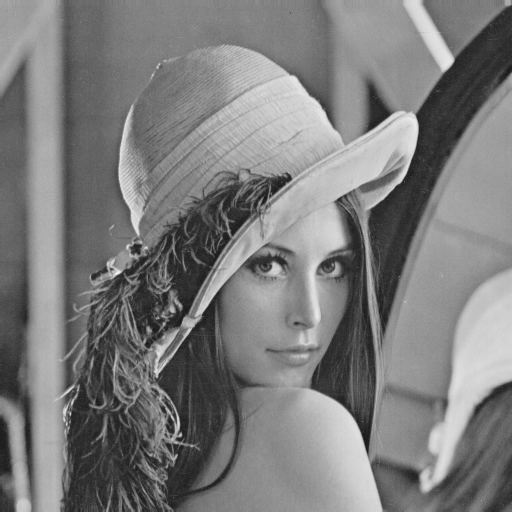
\includegraphics[height=9cm]{ej1-imgs/lena-original.png}
  \caption{\texttt{lena.png}}
\end{figure}

\begin{figure}[H]
\centering
\begin{subfigure}{0.5\linewidth}
\centering
  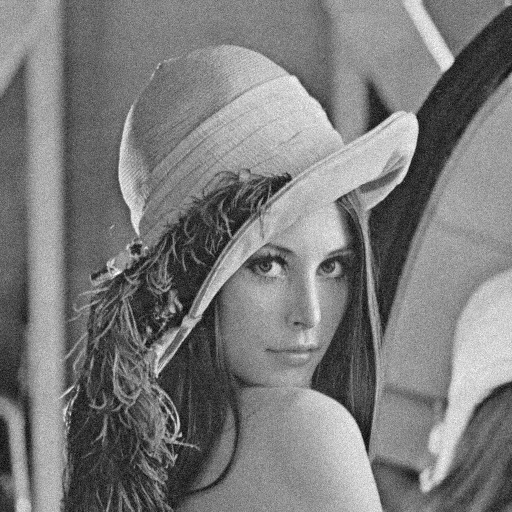
\includegraphics[height=9cm]{ej1-imgs/lena-gauss10.png}
  \caption{\footnotesize{\texttt{lena.png} con ruido gaussiano de media 10.}}
\end{subfigure}%
\begin{subfigure}{0.5\linewidth}
\centering
  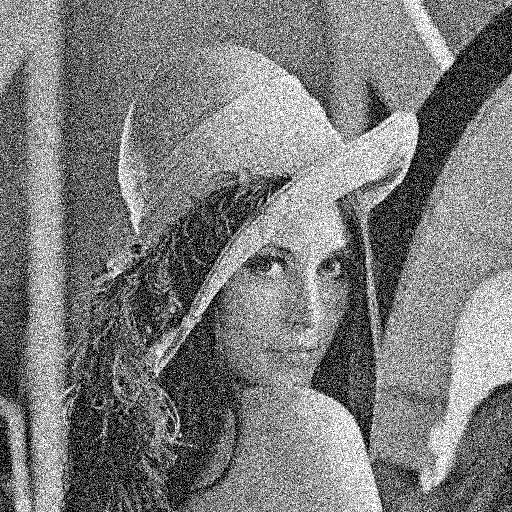
\includegraphics[height=9cm]{ej1-imgs/lena-gauss50.png}
  \caption{\footnotesize{\texttt{lena.png} con ruido gaussiano de media 50.}}
\end{subfigure}
\end{figure}

\begin{figure}[H]
\centering
\begin{subfigure}{0.5\linewidth}
\centering
  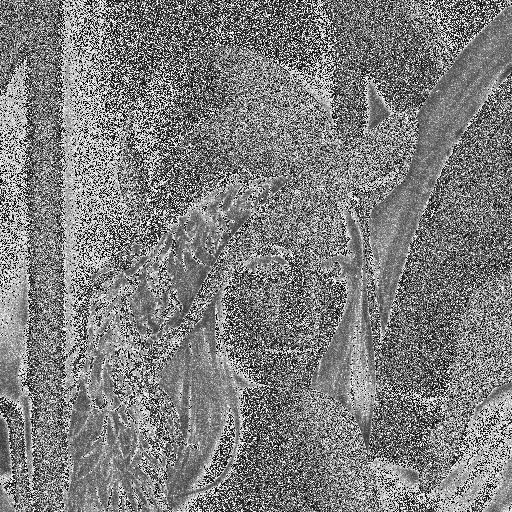
\includegraphics[height=9cm]{ej1-imgs/lena-rayleigh15.png}
  \caption{\footnotesize{\texttt{lena.png} con ruido rayleigh de parámetro 1.5.}}
\end{subfigure}%
\begin{subfigure}{0.5\linewidth}
\centering
  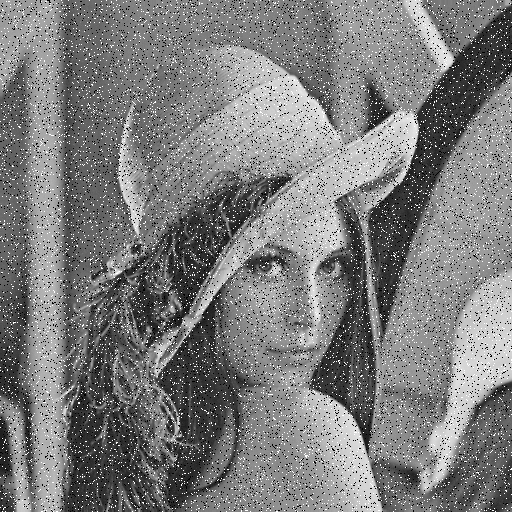
\includegraphics[height=9cm]{ej1-imgs/lena-saltpepper10.png}
  \caption{\footnotesize{\texttt{lena.png} con ruido salt \& pepper con probabilidad 0.1}}
\end{subfigure}
\end{figure}


\begin{figure}[H]
\centering
  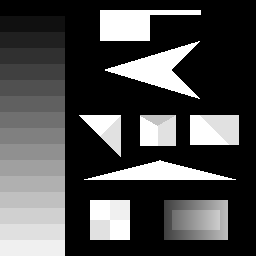
\includegraphics[height=9cm]{ej1-imgs/test-original.png}
  \caption{\texttt{test.png}}
\end{figure}

\begin{figure}[H]
\centering
\begin{subfigure}{0.5\linewidth}
\centering
  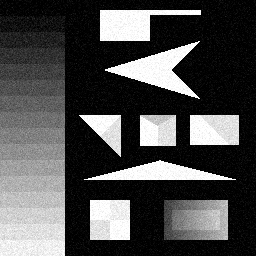
\includegraphics[height=9cm]{ej1-imgs/test-gauss10.png}
  \caption{\footnotesize{\texttt{test.png} con ruido gaussiano de media 10.}}
\end{subfigure}%
\begin{subfigure}{0.5\linewidth}
\centering
  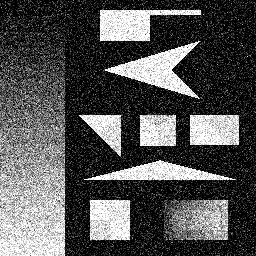
\includegraphics[height=9cm]{ej1-imgs/test-gauss50.png}
  \caption{\footnotesize{\texttt{test.png} con ruido gaussiano de media 50.}}
\end{subfigure}
\end{figure}

\begin{figure}[H]
\centering
\begin{subfigure}{0.5\linewidth}
\centering
  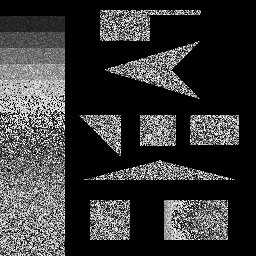
\includegraphics[height=9cm]{ej1-imgs/test-rayleigh15.png}
  \caption{\footnotesize{\texttt{test.png} con ruido rayleigh de parámetro 1.5.}}
\end{subfigure}%
\begin{subfigure}{0.5\linewidth}
\centering
  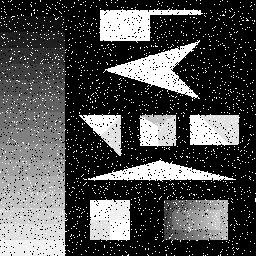
\includegraphics[height=9cm]{ej1-imgs/test-saltpepper10.png}
  \caption{\footnotesize{\texttt{test.png} con ruido salt \& pepper con probabilidad 0.1}}
\end{subfigure}
\end{figure}



\end{document}
